\documentclass[12pt, letterpaper]{article}
\usepackage[utf8]{inputenc}
\usepackage{setspace}
\usepackage{subcaption} 
\usepackage{hyperref}
\usepackage{float}
\usepackage{url}
\usepackage{amsthm}
\usepackage{graphicx}
\usepackage{amssymb}
\usepackage{amsmath}
\usepackage[lastexercise]{exercise}
\usepackage{tikz}
\usetikzlibrary{matrix}
\graphicspath{{images/}} \newtheorem{definition}{Definition}[section] \newtheorem{theorem}{Theorem}[section]
\newtheorem{corollary}{Corollary}[theorem]
\newtheorem{lemma}[theorem]{Lemma}
\newcommand{\R}{\mathbb{R}}
\newcommand{\Z}{\mathbb{Z}}
\newcommand{\implies}{\Rightarrow}
\title{Morse Theory}
\author{Veronika Starodub \\ Miloš Vukadinović \\ Nikolay Ninov} \date{\today } 
\doublespacing
\begin{document} 
\maketitle

\begin{figure}[h]
    \centering
    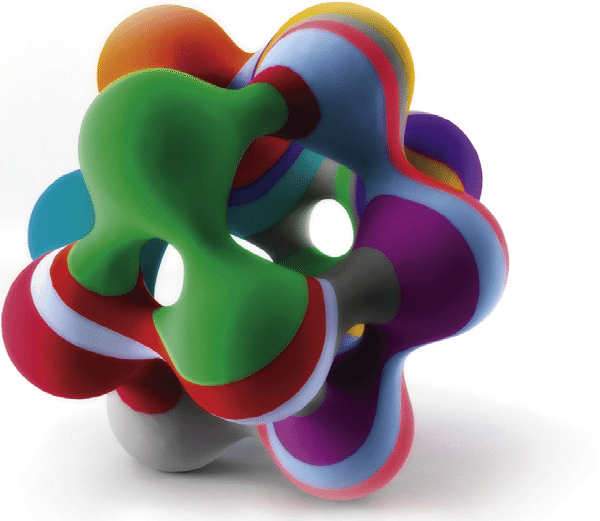
\includegraphics[width=0.50\textwidth]{cover}
\end{figure}
 
\tableofcontents
\section{Introduction}
\begin{document}

    \paragraph{\textbf{Morse Lemma.}}
        Suppose that the point $a \in \mathbb{R}^k$ is a nondegenerate
        critical point of the function $f$, and
        $$
            (h_{ij})= \left(  \frac{\partial^2f}{\partial x_i \partial x_j} (a) \right)
        $$
        is the Hessian of $f$ at $a$. Then there exists a local coordinate system
        $(x_1,\ldots,x_k)$ around $a$ such that
        $$
            f=f(a)+\sum{h_{ij}x_ix_j}
        $$
        near $a$.
        \\
        or
        $$
            f=-x_1^2-x_2^2-\ldots-x_\lambda^2+x_\lambda^2+\ldots+x_n^2+f(a)
        $$
        where $\lambda$ is the index of $f$ at $a$.

    \paragraph{\textbf{Theorem 1.1}} \textit{ 
        Let $f$ be a smooth function in a neighborhood 
    $N_x$ of $x=(x_1,\ldots,x_n)$ in $\mathbb{R}^n$. Suppose $f(0,\ldots,0)=0$. Then, 
    there exist $n$ smooth functions $g_i,\ldots,g_n$ defined on $N_x$ such that $g_i(0,\ldots,0)=\frac{\partial f}{\partial x_i}(0,\ldots,0)$
    for every $i$, and
    }

    $$
        f(x_i,\ldots,x_n)=\sum_{i=1}^{n}{(x_i,\ldots,x_n)}
    $$

    \paragraph{\textbf{Theorem 1.2}} \textit{ (Inverse Function Theorem)
        Let $f:\mathbb{R}^n\to \mathbb{R}^n$ be a smooth function on an open set $U$
        containing $a\in\mathbb{R}^n$. Suppose that $\det J_f(a)\not = 0$.
        \\Then there is an open set $V \subset \mathbb{R}^n$ containing $a$ and an open
        set $W\subset \mathbb{R}^n$ containing $f(a)$ such that $f:V\to W$ is a 
        diffeomorphism.
    }

    \paragraph{\textbf{Proof.}} Let $p_0$ be a nondegenerate critical point of the function
     $f:\ M \to \mathbb{R}$, where $M$ is an $n$-manifold. The degeneracy of the point
     $p_0$ on $f$ is determined independent of our choice of a local coordinate system.
     Therefore, we may assume that when we pick a local coordinate system $(x_1,\ldots,x_n)$ defined
     in a neighborhood $N_{p_0}$,

     \begin{equation}
        \frac{\partial^2f}{\partial x_1^2}(p_0)\not = 0\tag{1.1}
     \end{equation}

    or that we may pick a suitable linear transformation of the local coordinate
    system such that equation $1.1$ is true. We may further assume that $p_0$ corresponds
    to the origin $(0,\ldots,0)\in \mathbb{R}^n$ on the local coordinate system and that $f(p_0)=0$,
    replacing $f$ with $f-f(p_0)$ if necessary.
    
    By Theorem 1.1, there exit $n$ smooth functions $g_i,\ldots,g_n$ defined on
    $N_{p_0}$ such that

     \begin{equation}
        g_i(0,\ldots,0)=\frac{\partial f}{\partial x_i}(0,\ldots,0) \tag{1.2}
     \end{equation}

     and

     \begin{equation}
        f(x_1,\ldots,x_n)=\sum_{i=1}^{n}{(x_1,\ldots,x_n)}\tag{1.3} 
     \end{equation}

     But since $p_0$ is a critical point, equation $1.2$ turns out to be zero on both 
     sides at $p_0$. So we can apply Theorem $1.1$ again to get $n$ smooth functions 
     $h_{i1},\ldots,h_{in}$ for every $i$ that is defined on $N_{p_0}$ such that

     \begin{equation}
        \sum_{j=1}^{n}{x_jh_{ij}(x_1,\ldots,x_n)}=g_i(x_1,\ldots,x_n) \tag{1.4}
     \end{equation}

     By plugging equation $1.4$ into equation $1.3$, we get

     \begin{equation}
        f(x_1,\ldots,x_n)=\sum_{i=1}^{n}\sum_{j=1}^{n}{x_ix_jh_{ij}(x_1,\ldots,x_n)} \tag{1.5}
     \end{equation}

     We may assume that $h_{ij}=h_{ji}$, rewriting $h_{ij}$ as
     $H_{ij}=\frac{h_{ij}+h_{ji}}{2}$ if necessary. Furthermore,

     \begin{equation}
        (h_{ij}(0,\ldots,0))_{n \times n}=\left( \frac{1}{2}\frac{\partial^2f}{\partial x_i \partial x_j}(0,\ldots,0)_{n\times n} \right) \tag{1.6}
     \end{equation} 
     And since we assumed equation $1.1$ to be true, then $h_{11}(0,\ldots,0)\not = 0$. $h_{11}$
     is a smooth, hence continuous function, and so $h_{11}$ is not zero in a neighborhood of the origin.
     Let us call this neighborhood $\bar{N}_0$    

     Our ultimate goal is to express $f$ in the standard quadratic form of the equation from the lemma.
     We do this by eliminating all terms which are not of the form $\pm x_i^2$ via induction over $k\le n$
     steps. While we are currently dealing with $k=1$, in the general case of $k$, we wish to express $f$ 
     as a sum of terms such that $k$ terms are of the form $\pm x_i^2$ and the rest of the terms depend
     on coordinate in the set ${x_i|i\not = k}$. To this end, let
     \begin{equation}
        G(x_1,\ldots,x_n)=\sqrt{|h_{11}(x_1,\ldots,x_n) | }   \tag{1.6}
     \end{equation}
        
     G is a smooth, non-zero function of $x_1,\ldots,x_n$ on $\bar{N}_0$.

     Now suppose by induction that there exists a local coordinate system $(y_1,\ldots,y_n)$ defined on $\bar{N}_0$ such that
     \begin{equation}
        y_i=x_i(\not = 1) \tag{1.7}
     \end{equation}
     \begin{equation}
        y_1=G*(x_1+\sum_{i>1}^{n}{\frac{x_ih_{1i}}{h_{11}}})\tag{1.8}
     \end{equation}

     It follows from the Inverse Function Theorem that $y_1,\ldots,y_n$ is a local
     coordinate system defined on a smaller neighborhood $\tilde{N}_0 \subset \bar{N}_0$,
     since the determinant of the Jacobian of the transformation from $(x_1, \ldots,x_n)$
     to $(y_1,\ldots,y_m)$ may be verified to be nonzero.

     When we square $y_1$, we get
     \begin{equation}
        y_1^2=\pm h_{11}x_1^2\pm2\sum_{i=2}^{n}{x_1x_ih_{1i}}\pm\frac{\left(\sum_{i=2}^{n}{x_ih_{1i}}\right)^2}{h_{11}}\tag{1.9}
     \end{equation}
     where the signs are either positive or negative, depending on the sign of $h_{11}$. Using equation
     $1.5$, we can verify that $f$ can be expressed in the following way with respect to this
     coordinate system on the restricted domain $\tilde{N}_0$.
     \begin{equation}
        f=\pm y_1^2 + \sum_{i=2}^{n}\sum_{j=2}^{n}{x_ix_jh_{ij}}-\frac{\left(\sum_{i=2}^{n}{x_ih_{1i}}\right)^2}{h_{11}}\tag{1.10}
     \end{equation}
     where the sign of the $y_1^2$ term is positive or negative, depending on the sign of $h_{11}$. Staying
     consistent with our goals, we notice that the first term is in the standard quadratic form seen
     in the Morse Lemma formulation, whereas the rest of the terms depend on local coordinates
     $x_i$ whereby $i\not=k \ (k=1)$. By induction from $k=1$ to $k=n$, we prove the Morse Lemma. $\blacksquare$

\textbf{Ex.} Show that the function $f: S^2 \to \R, f(x,y,z) = z$ is a Morse function. \\

$f$ is smooth on $ S^2 $ since it extends to a smooth map on all of $\R^3$. We can map $R^3$ to $S^2$ with the stereographic projection two functions:\\
$
	\phi_1(x_1,x_2,x_3) = (\frac{x_1}{1-x_3}, \frac{x_2}{1-x_3} ) 
$
and
$
	\phi_2(y_1,y_2,y_3) = (\frac{y_1}{1+y_3},\frac{y_2}{1+y_3})
$\\
Therefore, to get $S^2 \to R^3$ we can take $\phi_1^{-1}$ and $\phi_2^{-1}$ \\
$
	\phi_1^{-1}(x_1,x_2,x_3) = (\frac{2x_1}{x_1^2+x_2^2+1}, \frac{2x_2}{x_1^2+x_2^2+1}, \frac{x_1^2+x_2^2-1}{x_1^2+x_2^2+1})
$\\
$
	\phi_1^{-1}(y_1,y_2,y_3) = (\frac{2y_1}{y_1^2+y_2^2+1}, \frac{2y_2}{y_1^2+y_2^2+1}, \frac{1-y_1^2+y_2^2}{y_1^2+y_2^2+1})
$\\
Then, we take $g_1 = f \circ \phi_1^{-1}$ and $g_2 = f \circ \phi_2^{-1}$ \\
$
	g_1(x,y) =  \frac{x^2+y^2-1}{x^2+y^2+1}
$
and
$
	g_2(x,y) = \frac{1-x^2+y^2}{x^2+y^2+1}
$ \\
Now, we can compute jacobian of $g_1$ and $g_2$, find critical points, and check that determinant of hessian matrix is non-zero. \\
$
	\nabla g_1(x,y,z) = 0$ iff $(x,y,z) = (0,0,-1)
$\\
$
	\nabla g_2(x,y,z) = 0$ iff $ (x,y,z) = (0,0,1)
$
We have two critical points, and now we compute the hessian at them.\\
$
	H(g_1) = \begin{bmatrix} 4 & 0 \\ 0 & 4 \end{bmatrix}
	\implies \det(H(g_1)) = 16
$\\
$
	H(g_2) = \begin{bmatrix} -4 & 0 \\ 0 & -4 \end{bmatrix}
	\implies \det(H(g_2)) =  16

$\\ 

Both critical points are non-degenerate, therefore $f$ is a Morse function.$\blacksquare$\\
\\
\\
Examples of Morse functions: \\
\textbf{Example 1.1}\\
$f(x,y)=e^{xy}+x$\\
First of all we have to find all critical points of $f$. A point $P$ is critical, when $\frac{\partial f}{\partial x}=\frac{\partial f}{\partial y}=0$ at $P$. \\
$\frac{\partial f}{\partial x}= ye^{xy}+1=0 \\
\frac{\partial f}{\partial y}=xe^{xy}=0$
After solving the system of equations we get that $x=0$, $y=-1$. Hence, the only critical point of $f$ is $(0,-1)$. Now to prove that the function is a Morse function we have to shoe that the determinant of Hessian matrix at the point $(0,-1)$ is non-zero. \\
Partial second order derivatives are: \\
$\frac{\partial^2 f}{\partial x^2}=y^2e^{xy}$
$\frac{\partial^2 f}{\partial x^2}(0,-1)=1$\\
$\frac{\partial^2 f}{\partial \partial y}=e^{xy}+yxe^{xy}$
$\frac{\partial^2 f}{\partial \partial y}(0,-1)=1$\\
$\frac{\partial^2 f}{\partial y \partial x}=e^{xy}+xye^{xy}$
$\frac{\partial^2 f}{\partial y \partial x}(0,-1)=1$\\
$\frac{\partial^2 f}{\partial y^2}=x^2e^{xy}$
$\frac{\partial^2 f}{\partial y^2}(0,-1)=0$\\
Therefore, \\
$det(Hess(f(0,-1)))=\left| \begin{array}{cc} 1 & 1 \\ 1 & 0 \end{array} \right|=-1$. \\
Since the determinant is non-zero at the only critical point of the function, we can claim that it is a Morse function. \\
\textbf{Example 1.2}\\
Let's consider a function $g(x,y)=xy$ and prove that it is , indeed, a Morse function.\\
First order partial derivatives: \\
$\frac{\partial g}{\partial x}=y$\\
$\frac{\partial g}{\partial y}=x$\\
Therefore, the only critical point of $g$ is $(0,0)$. Now we have to evaluate the determinant of Hessian matrix at this point.\\
Second order partial derivatives: \\
$\frac{\partial^2 g}{\partial x^2}=0$\\
$\frac{\partial^2 g}{\partial x \partial y}=1$\\
$\frac{\partial^2 g}{\partial y \partial x}=0$\\
$\frac{\partial^2 g}{\partial^2 y}=1$\\
Hence the determinant of Hessian at the critical point is: \\
$det(Hess(f(0,0)))=\left| \begin{array}{cc} 0 & 1 \\ 1 & 0 \end{array} \right|=-1$. \\
We observe that the determinant is nonzero, hence, the only critical point of $g(x,y)=xy$ is non-degenerate, so the function is Morse. \\
\\
\\
Examples of functions that are not Morse: \\
\textbf{Example 2.1}\\
$f(x,y)=x^3+xY^2-x^2y-y^3$\\
Let's follow the previous procedure: \\
$\frac{\partial f}{\partial x}=3x^2+y^2-2xy=0$\\
$\frac{\partial f}{\partial y}=2xy-x^2-3y^2=0$\\
After solving the system of equations we got that the only critical point of $f$ is $(0,0)$. Now compute second order partial derivatives:\\
$\frac{\partial^2 f}{\partial x^2}=6x-2y$\\
$\frac{\partial^2 f}{\partial x \partial y}=2y-2x$\\
$\frac{\partial^2 f}{\partial y \partial x}=2y-2x$\\
$\frac{\partial^2 f}{\partial^2 y}=2x-6y$\\
Therefore, \\
$det(Hess(f(0,0)))=\left| \begin{array}{cc} 0 & 0 \\ 0 & 0 \end{array} \right|=0$.\\
Hence, the only critical point of $f$ is degenerate, so $f$ is not a Morse function. \\
\textbf{Example 2.2}\\
$g(x,y)=x^3$\\
$\frac{\partial g}{\partial x}=3x^2$\\
$\frac{\partial g}{\partial y}=0$\\
Therefore, critical points are all points of the form $(0, y_1)$.\\
$\frac{\partial^2 g}{\partial x^2}=6x$
$\frac{\partial^2 g}{\partial x \partial y}=0$\\
$\frac{\partial^2 g}{\partial y \partial x}=0$
$\frac{\partial^2 g}{\partial^2 y}=0$\\
Hence, Hessian will be of the form: \\
$Hess(g(0,y_1))=\left| \begin{array}{cc} 0 & 0 \\ 0 & 0 \end{array} \right|,  \forall y_1$. \\
Therefore, all critical points of $g$ are degenerate points, moreover, values of $g$ at all critical points are equal, hence, $g(x,y)=x^3$ is not a Morse function. 


\end{document}
